\documentclass[letterpaper]{article}
\usepackage{natbib,alifeconf,hyperref}

\title{The Pop Button}
\author{Kentin$^{1}$, Cl\'emence$^{2}$, Nil$^{3}$ \and Florian$^4$}



\begin{document}
\maketitle

\section{In a word}

The pop button is a device that aim to be your daily companion for noting every fournitures you need anytime you think about it


\section{Introduction}

The device needs a 'rotate and push' button$^5$, a wi-fi module to communicate with a server, a screen, a battery holder and some other things that we no idea what it should be... 

\section{Block Diagram}

This is a basic block diagram describing the architecture of the device
\begin{figure}[!htb]
\begin{center}
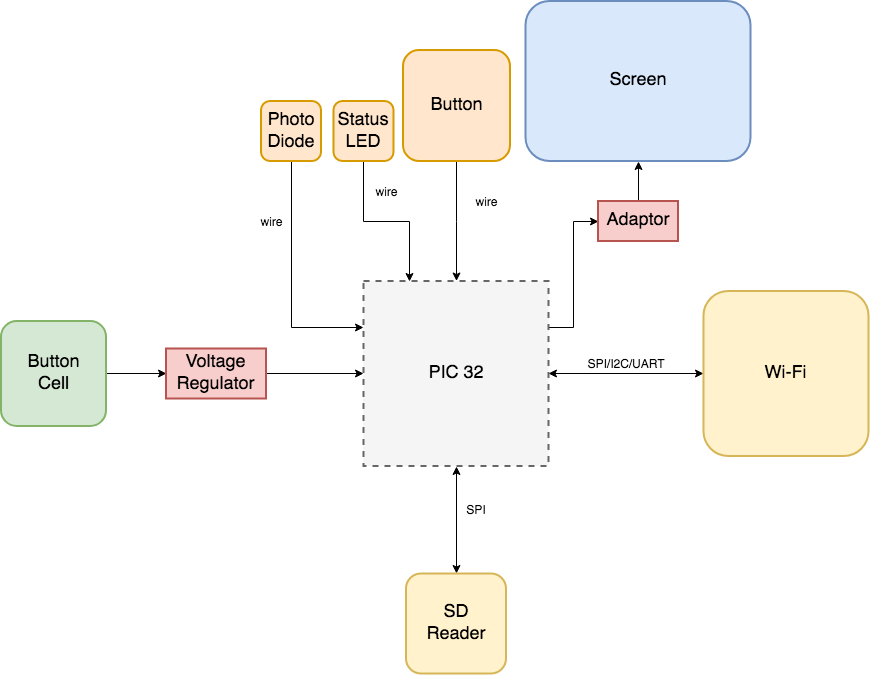
\includegraphics[width=3in]{test_img_block_diagram.png}
\caption{Sample picture caption.}
\label{fig1}
\end{center}
\end{figure}

I love writing things

\begin{table}[!hbt]
\center{
\begin{tabular}{|c|c|c|}\hline
One & Two & Three\\ \hline\hline
Yes & 0 & 1 \\
Not  & 1 & 0 \\
Maybe & 0.5 & 0.5 \\ \hline
\end{tabular}
}
\vskip 0.25cm
\caption{Sample table caption.}
\end{table}

Lorem ipsum dolor sit amet, consectetur adipiscing elit, sed do eiusmod tempor incididunt ut labore et dolore magna aliqua. Ut enim ad minim veniam, quis nostrud exercitation ullamco laboris nisi ut aliquip ex ea commodo consequat. Duis aute irure dolor in reprehenderit in voluptate velit esse cillum dolore eu fugiat nulla pariatur. Excepteur sint occaecat cupidatat non proident, sunt in culpa qui officia deserunt mollit anim id est laborum. 

\footnotesize
\bibliographystyle{apalike}
\bibliography{sample}

{
\mbox{}\\
$^1$qdurot \\
$^2$clbergon\\
$^3$nburcion \\
$^4$fde-souz\\
$^5$\href{http://fr.farnell.com/bourns/pel12d-2226f-s3024/rotary-encoder-incremental-24/dp/1857558?st=rotary\%20encoder}{rottary button}\\
$^6$\href{http://fr.farnell.com/keystone/2480cn/battery-holder-aaa-size-wire-lead/dp/2784201?st=battery\%20holder}{battery holder}
}

\end{document}
